\documentclass[border=10pt]{standalone}

\usepackage{tikz}
\usepackage{tikzsymbols}
\usetikzlibrary{calc,patterns,shapes.geometric}

\def\centerarc[#1](#2)(#3:#4:#5){\draw[#1] ($(#2)+({#5*cos(#3)},{#5*sin(#3)})$) arc (#3:#4:#5);}

\begin{document}
	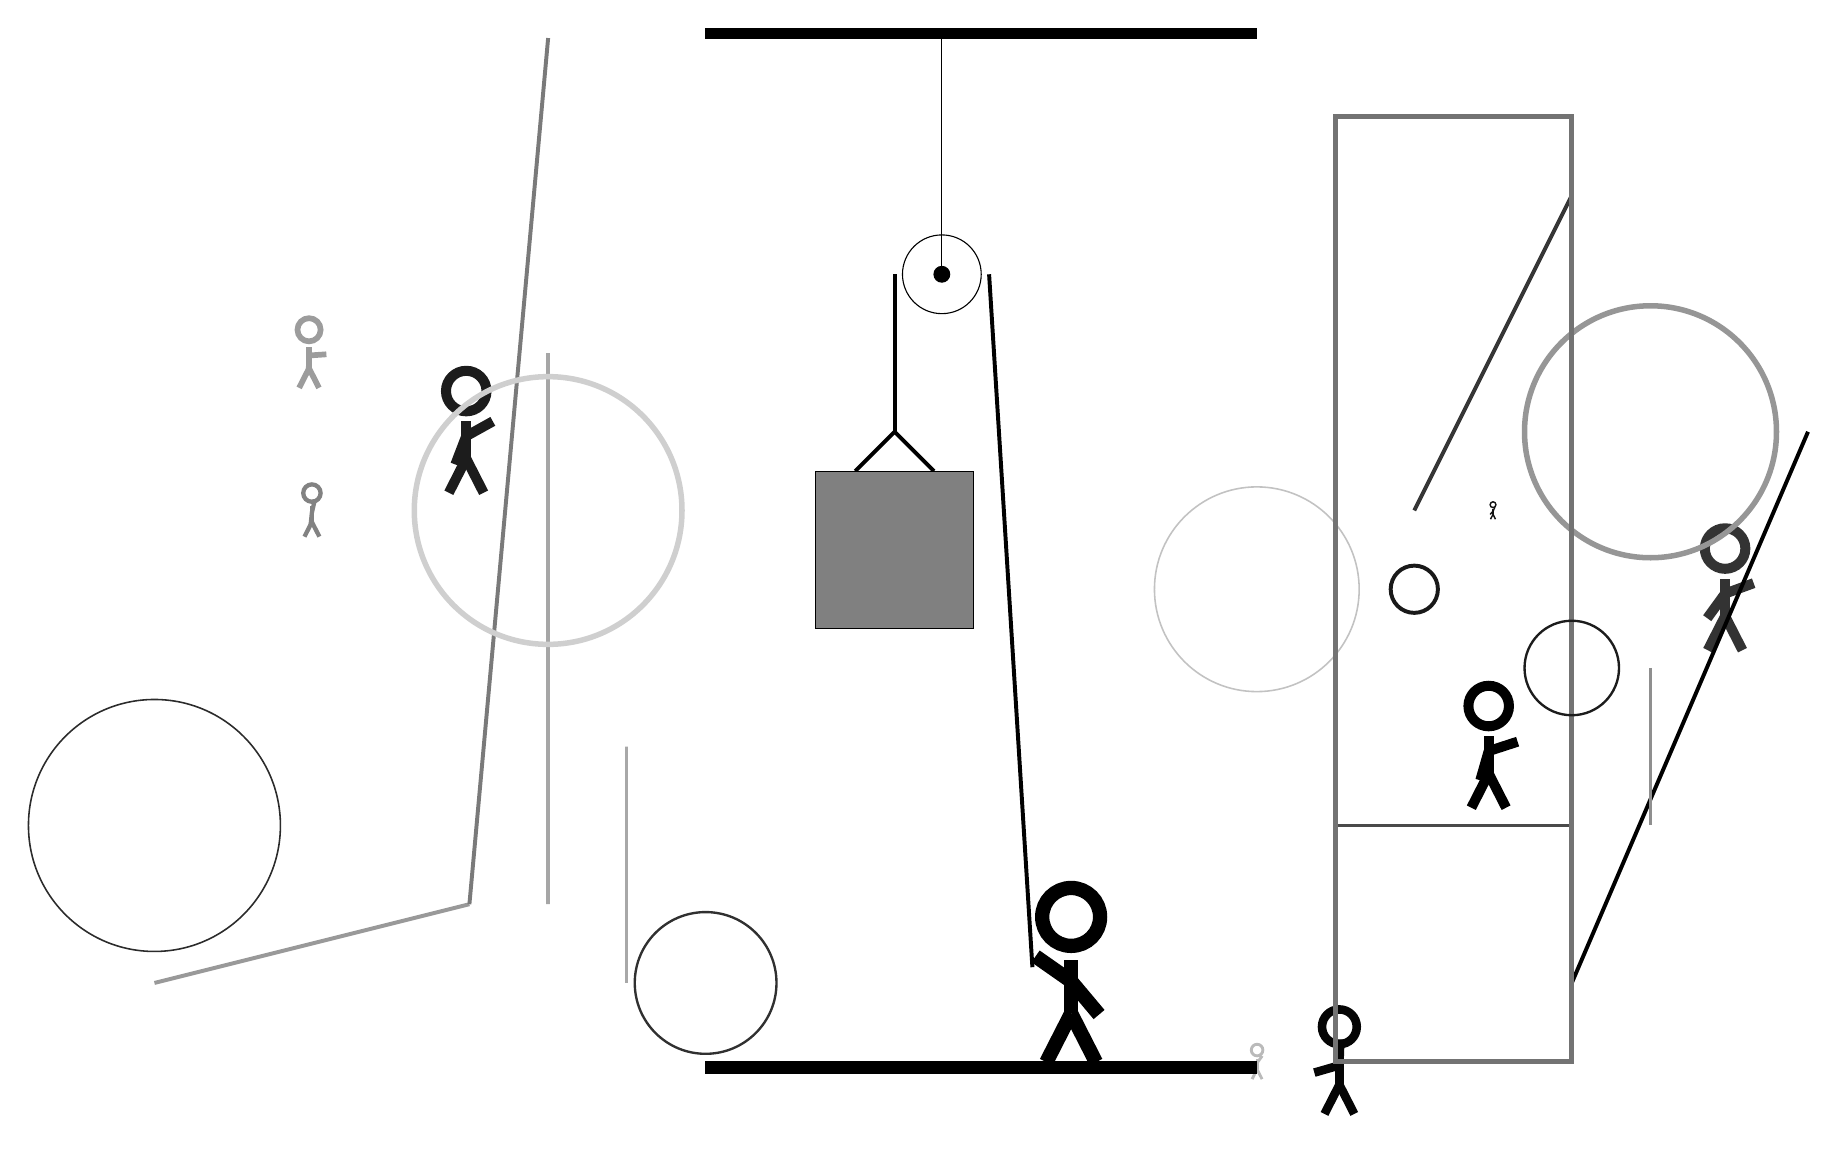
\begin{tikzpicture}
		%%%%% START %%%%%
		
		\draw[fill=black] (-2, 10) rectangle (5, 10.125);
		
		\draw (1, 7) circle (0.5);
		\draw[fill=black] (1, 7) circle (0.1);
		\draw (1, 10) -- (1, 7);
		
		\draw[line width=0.5mm] (-0.1, 4.5) -- (0.4, 5.0) -- (0.9, 4.5);
		\draw[fill=black!50] (-0.6, 4.5) rectangle (1.4, 2.5);
		
		\draw [line width=0.5mm, color=black!90](7, 3) circle (0.3);
		
		\node[line width=0.4mm, color=black!80] at (11, 3) {\Strichmaxerl[7][54][20]};
		\node[line width=0.5mm, color=black!100] at (8, 1) {\Strichmaxerl[7][74][18]};
		\node[line width=0.5mm, color=black!39] at (-7, 6) {\Strichmaxerl[4][89][4]};
		\draw [line width=0.7mm, color=black!41](10, 5) circle (1.6);
		
		\draw[line width=0.5mm, color=black!100](9, -2) -- (12, 5);
		\draw[line width=0.5mm, color=black!44](10, 2) -- (10, 0);
		\node[line width=0.7mm, color=black!49] at (-7, 4) {\Strichmaxerl[3][84][77]};
		\node[line width=0.5mm, color=black!27] at (5, -3) {\Strichmaxerl[2][43][54]};
		\draw [line width=0.2mm, color=black!83](-9, 0) circle (1.6);
		\draw[line width=0.5mm, color=black!35] (-4, -1) rectangle (-4, 6);
		\node[line width=0.7mm, color=black!93] at (8, 4) {\Strichmaxerl[1][49][64]};
		\draw[line width=0.5mm, color=black!40](-5, -1) -- (-9, -2);
		\node[line width=0.6mm, color=black!98] at (6, -3) {\Strichmaxerl[6][16][88]};
		\node[line width=0.2mm, color=black!89] at (-5, 5) {\Strichmaxerl[7][69][29]};
		\draw[line width=0.5mm, color=black!79](7, 4) -- (9, 8);
		
		\draw[line width=0.4mm, color=black!71] (6, 9) rectangle (9, 0);
		\draw [line width=0.3mm, color=black!81](-2, -2) circle (0.9);
		\draw [line width=0.2mm, color=black!24](5, 3) circle (1.3);
		
		\draw [line width=0.3mm, color=black!91](6, 4) circle (0.0);
		\draw[line width=0.6mm, color=black!55] (6, -3) rectangle (9, 9);
		
		\draw[line width=0.5mm, color=black!52](-5, -1) -- (-4, 10);
		\draw [line width=0.7mm, color=black!19](-4, 4) circle (1.7);
		\draw[line width=0.4mm, color=black!34] (-3, 1) rectangle (-3, -2);
		\draw [line width=0.3mm, color=black!89](9, 2) circle (0.6);
		
		\draw[line width=0.5mm] (0.4, 7) -- (0.4, 5.0);
		\centerarc[line width=0.5mm](1, 7)(0:180:0.6);
		\draw[line width=0.5mm](1.6, 7) -- (2.15, -1.8);
		
		\node at (2.6, -1.9) {\Strichmaxerl[10][-35][-50]};
		
		\draw[fill=black] (-2, -3) rectangle (5, -3.15);
		
		%%%%% END %%%%%
	\end{tikzpicture}
\end{document}